\chapter{序論}

\section{はじめに}
2004年、国際ヒトゲノム解読プロジェクトによる完全長ヒトゲノム配列の解読完了宣言から今日までのおよそ10年、分子生物学はゲノム、トランスクリプトーム、プロテオーム、メタボロームなどに代表されるオミックス科学がその全盛を極め、ENCODEやFANTOM、1000 Genomes Projectなど巨大な国際プロジェクトが今なお進行している。"Omics"はギリシャ語で「全体」や「総体」を意味し、オミックス科学は、DNAやRNA、タンパク質といった生命における異なる階層における地図を作ること、また複数の地図からボトムアップに生命現象を理解することを標榜する営みであると言えるだろう。特にここ数年、超並列シーケンサー (High-throughput sequencing)と呼ばれる高出力な配列決定技術の躍進は著しく、真核生物における遺伝子発現や転写機構について、高い定量性と広いダイナミックレンジを併せ持った観測を可能にしてきた。
\par
本研究は、こういった高出力かつ定量的なオミックスデータを背景とし、転写後修飾の一種であるRNA editingと呼ばれる現象に焦点を絞った研究である。目的は、大きく2つあり、一つは、RNA-seqデータからRNA editingサイトを検出するための情報学的な手法の開発、2つはヨコヅナクマムシにおけるRNA editingの解析である。

\section{真核生物におけるRNA editing}
\subsection{ADARによるA-to-I editing}
転写はゲノム上にコードされた遺伝情報を正確にコピーする機構である。転写は核内で起こる生化学反応であり、RNAポリメラーゼよって触媒される。転写された一本のpre-mRNAはスプライシングを受けイントロン領域が切りだされ、ポリアデニル化と5'キャップ付加を受けて成熟した後に、核膜孔を通して細胞質へ輸送される、というのが転写機構の大まかな素描である。ヒトゲノムの解読前、遺伝子数はおよそ10万個だと見積もられていたが、解読の完了によって2.5万個程度に大きく下方修正され、直感的な生命の複雑性とゲノムサイズや遺伝子数には相関関係が見られないことは今日に繰り返すまでもない。今日までの研究によって、真核生物の見せる多様性で複雑なシステムの多くは、転写後および翻訳後の転写物やタンパク質への修飾によって大部分が担保されていることが明らかとなってきた。細胞の内外の情報伝達の多くは、キナーゼによるタンパク質のカスケード的なリン酸化が引き金となり、転写因子が特定の遺伝子発現を制御する。このように、真核生物においては、前述した転写の素描に加え、有限個の遺伝子にその多様性を規定されながらも、転写後修飾および翻訳後修飾によって、転写物レベルあるいはタンパクレベルでの多様性や複雑性を保証する戦略を進化させてきたと考えられる。
\par
本研究は転写後修飾のとして最もよく知られるRNA editingと呼ばれる現象に着目している。RNA editingは転写物への一塩基修飾を指し、鞭毛虫のミトコンドリアRNAから初めて発見された。真核生物では、アデニン(A)からイノシン(I)へ修飾されるA-to-I editingの他に、シトシン(C)からチミン(T)への修飾がこれまで報告されている。植物においてはT-to-C editing、ヒトやマウス、ショウジョウバエなど高等真核生物においてはA-to-I editingが優勢を占めることが多くの研究から明らかになっている。
\par
しかしながら、アミノ酸配列の変化を伴うA-to-I editingの報告例は非コード領域におけるeditingに対して著しく少なく、非翻訳領域 (Untranslated regions, UTRs)やAlu配列といったイントロン内のレトロトランスポゾン領域におけるA-to-I editingが優勢を占めていることが明らかになっている。加えて、miRNAやRNAi経路とのクロストークを介したグローバルな遺伝子発現制御との関係性などが指摘されていることから、真核生物におけるA-to-I editingを理解するためには、non-coding RNAにおけるA-to-I editingを研究することが極めて重要であると言える。
から、non-coding RNAへのeditingを介した遺伝子発現制御にA-to-I editingが介在し、制御しうる可能性が徐々に明らかになりつつある。
すなわち、真核生物におけるRNA editingの理解には、従来想定されてきたようなアミノ酸置換を伴ったコード領域内へのeditingのみならず、非コード領域におけるeditingを研究し、その意味を理解することの重要性を示している。本論はこの視点に立脚し、RNA editing研究に関する最新の研究成果を出来うる限り盛り込むようなレビューに努めると同時に、今後のediting研究の進むであろう一つの方向性を示すことができればと考える。

\subsection{ADARの作用機序}
ADAR (adenosine deaminase acting on RNA)は、二本鎖RNA結合タンパクの一種として知られ、相補鎖を形成した二本鎖RNAと選択的に結合し、イノシンへの置換を触媒する (A-to-I editing)。イノシンへと置換された塩基は、転写機構においてグアノシンとして認識される。Guanosine receptor-2 (GluR2)やSerotonin receptor-2C (5-HTR)など位置特異的なA-to-I editingにおいては、隣接するエクソン-イントロン境界における相補的な配列、ECS (Editing-site complamentary sequence)およびその二次構造の形成が不可欠であることが知られている。
\par
加えて、Glutamine receptor (GluR)においては、editingサイト毎にADAR1またはADAR2のどちらか一方に選択的にeditingされることが知られており、位置毎におけるADARの選択性は、ADARの持つdsRBDの数とドメイン間の配列長の相違によるADARと二本鎖RNAとの相互作用が異なることに起因するとの報告がある。

以下にADARによるRNA editingの概略を示す。
\begin{figure}[htbp]
	\begin{center}
		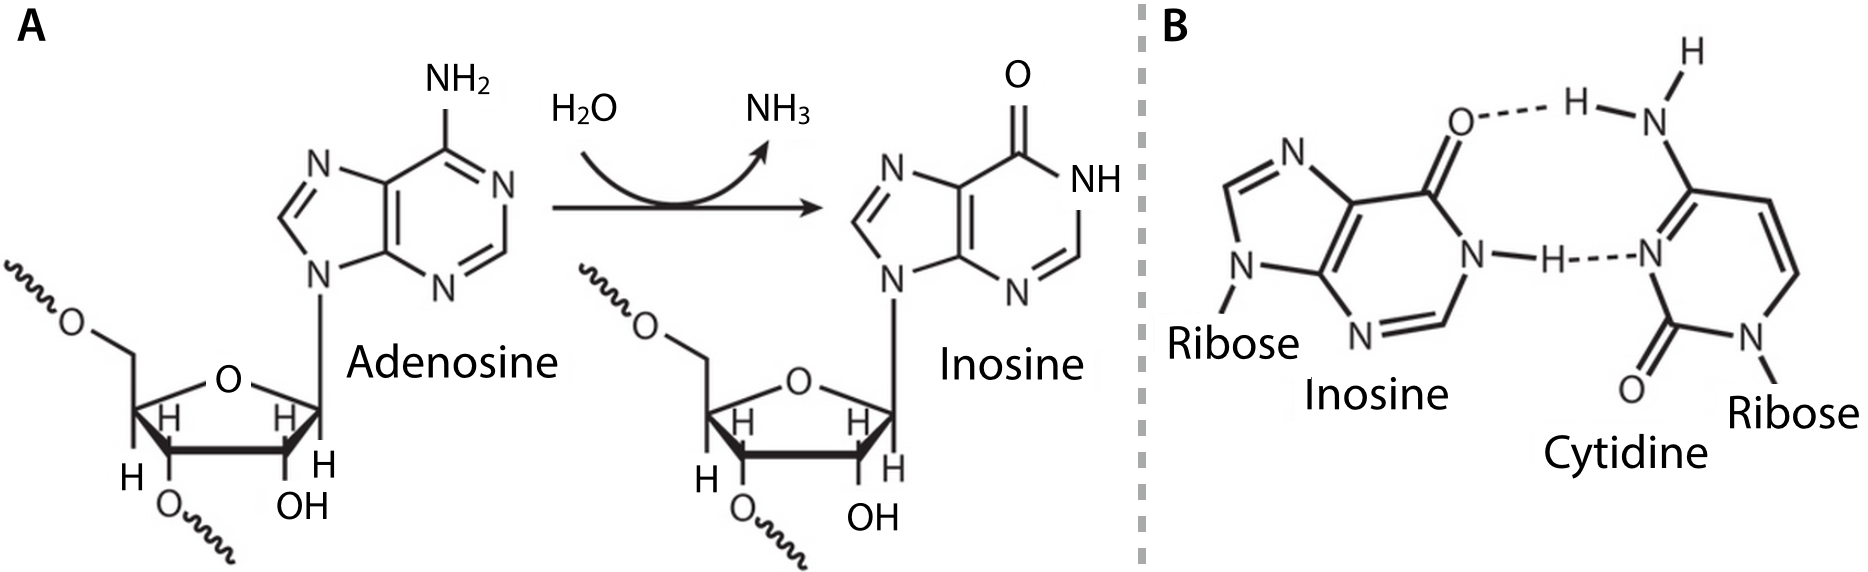
\includegraphics[width=14cm]{Adenosine-inosine.png}
	\end{center}
	\caption{ADARの生化学的な作用機序}
	\begin{flushleft}
		\normalsize{ADARによるアデノシンからイノシンへの化学修飾が触媒される様子を示す。}
	\end{flushleft}
	\label{fig:Chemical_reaction}
\end{figure}

\begin{figure}[htbp]
	\begin{center}
		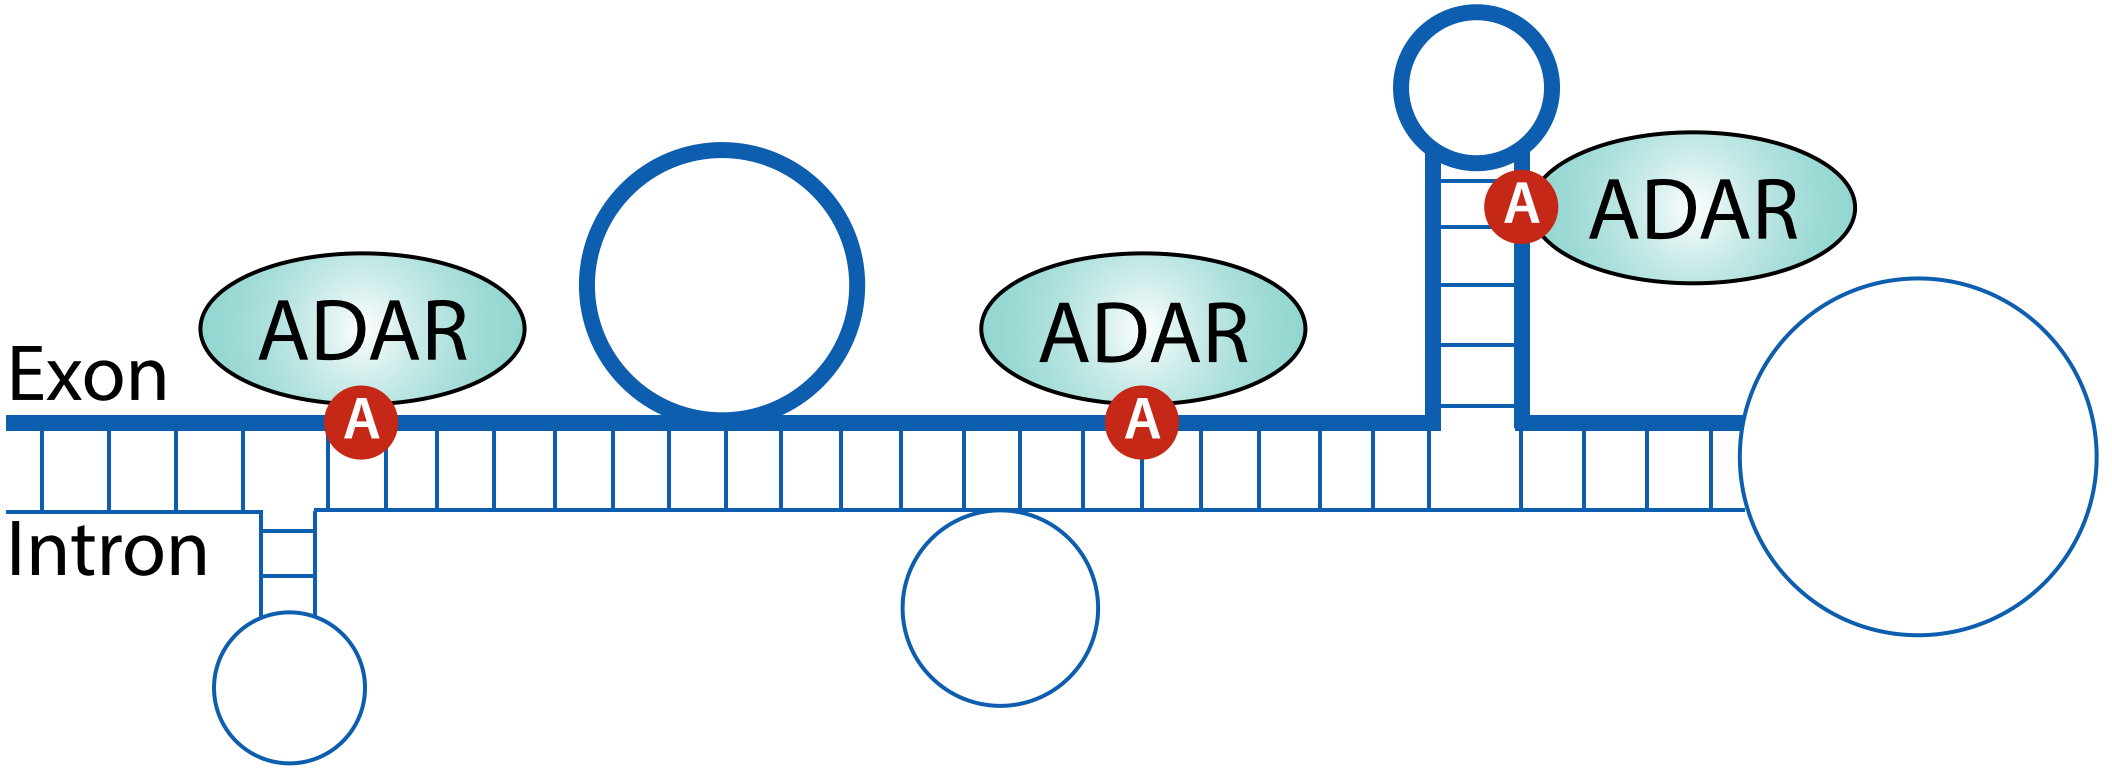
\includegraphics[width=14cm]{ADAR.png}
	\end{center}
	\caption{ADARの作用機序}
\end{figure}

\subsection{ADARのドメイン構造}
すべてのADARはA-to-I editingを触媒するdeaminaseドメインと二本鎖RNAに結合するdsRB (Double-strand binding)ドメインの2つを共通して有している。ヒトにおいては、これまでにADAR1、ADAR2、ADAR3の3種類が同定されており、そのうちADAR1については核内および細胞質に局在するADAR1LおよびADAR1Sが知られる他、ADAR3は脳特異的に発現することが知られている。ヒトにおけるADAR1およびADA2は、上記2つの機能ドメインの他にもZ-DNA結合ドメインを有している。

マウス、ショウジョウバエ、線虫におけるADARはバリアントが複数同定されている。

\begin{figure}[htbp]
	\begin{center}
		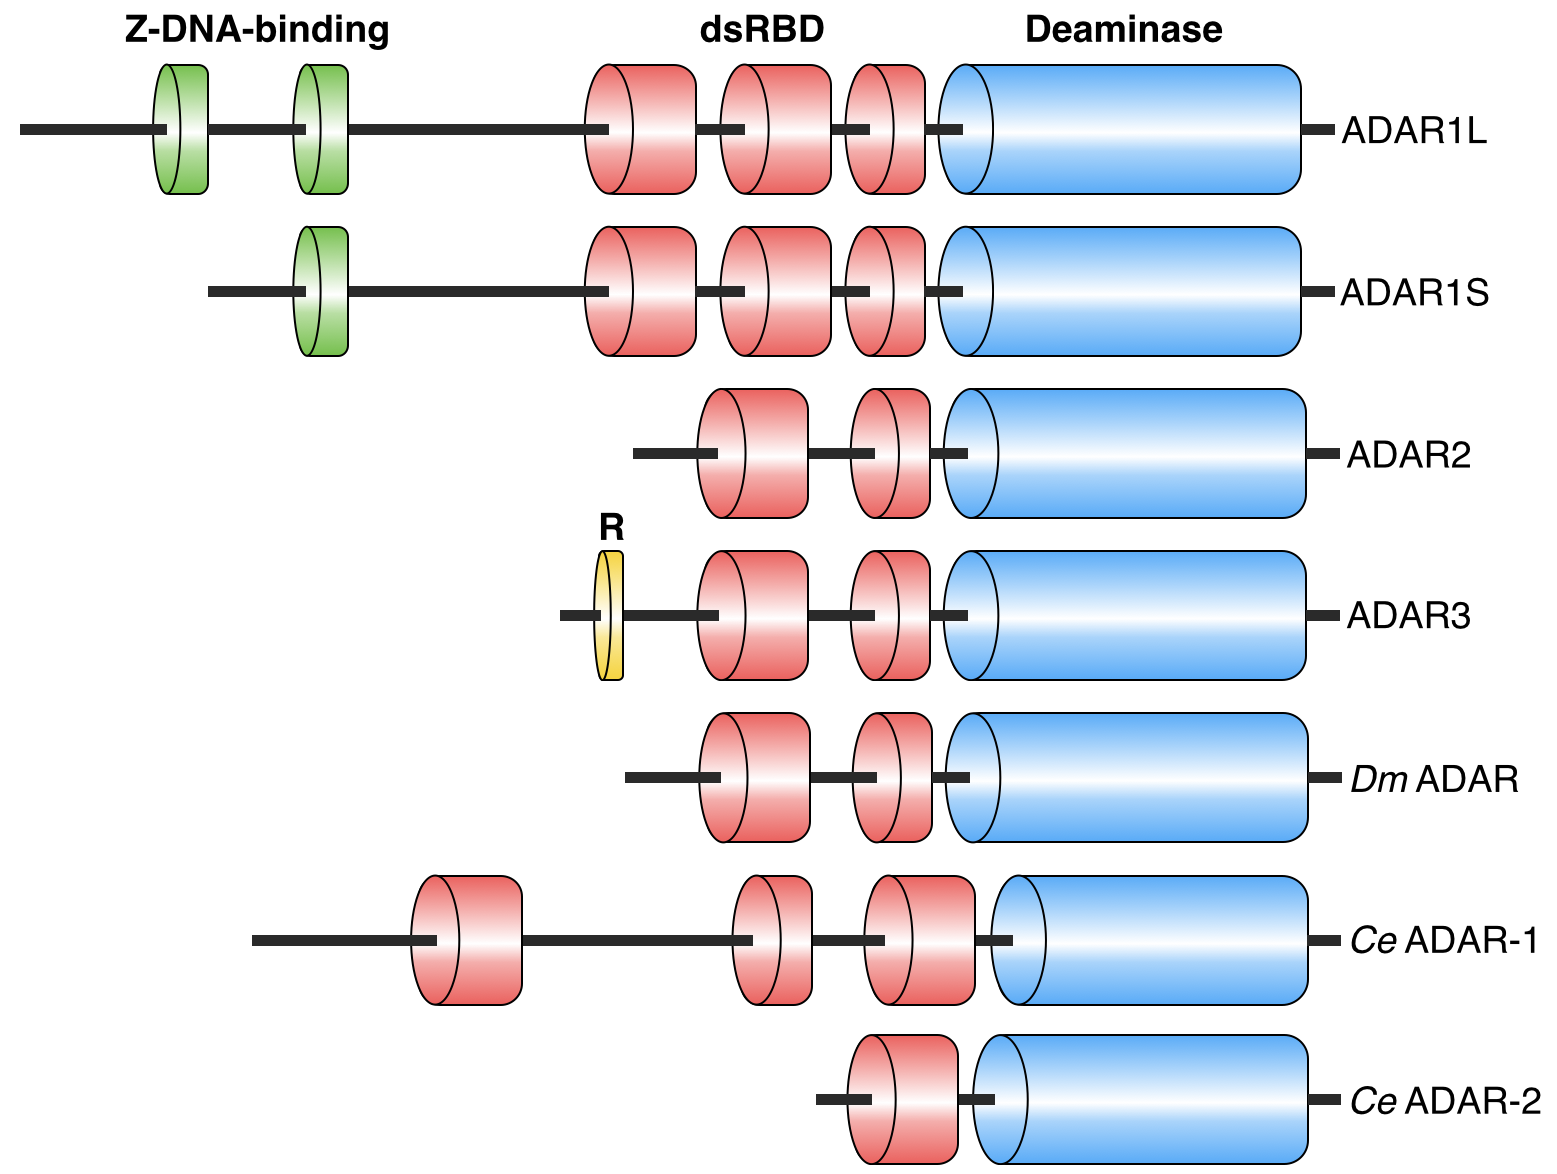
\includegraphics[width=14cm]{Adar_domain.png}
	\end{center}
	\caption{ADARのドメイン構造}
\end{figure}

\subsection{ADARの発現と細胞内局在}

\section{遺伝子領域におけるA-to-I editingとタンパクの多様化}

\section{非コード領域におけるA-to-I editing}
\subsection{反復配列におけるA-to-I editing}

\subsection{miRNAへのeditingと遺伝子発現制御}
\subsection{A-to-I editingとRNAiのクロストーク}
\subsection{A-to-I editingとスプライシングの関係性}

\section{情報学的解析によるRNA editingサイトの検出}
\subsection{超並列シーケンサーによる網羅的解析}
\subsection{検出手法の開発}
\subsection{組織およびセルライン特異的なRNA editing}

